\chapter{Implementation}
\label{chap:Implementation}
In this chapter the implementation of the language and the tool, the problems faced, and the solutions adopted will be discussed

\section{General overview of the tool}
\begin{figure}
    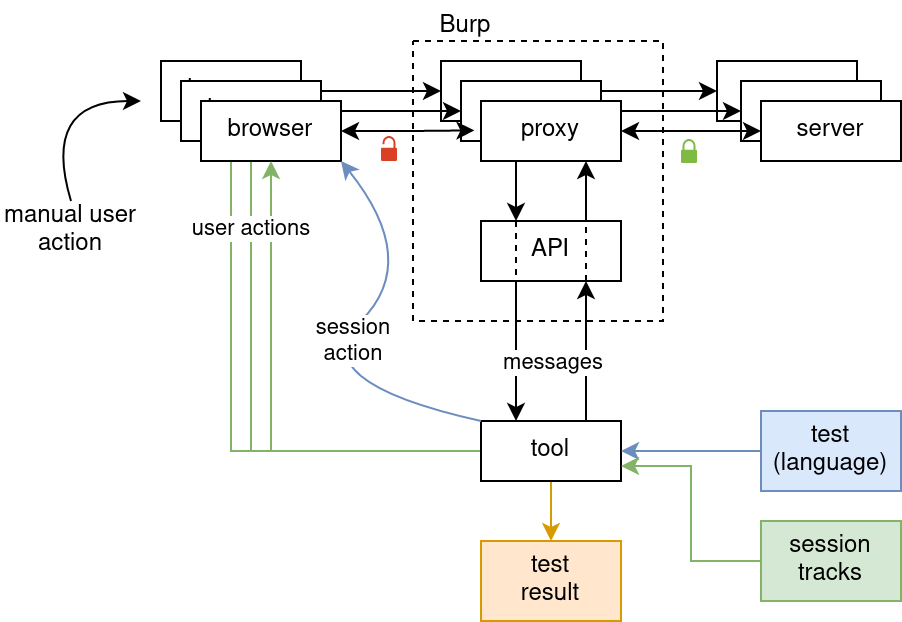
\includegraphics[width=\textwidth]{general_schema.png}
    \caption{General schema}
    \label{fig:general_schema}
\end{figure}

The components of the final tool can be seen in Figure \ref{fig:general_schema}. Burp Suite is composed by its proxy and related APIs, the tool will get all the messages from the proxy through the API, it will process them, and return them to the proxy. This way all the messages will pass through the tool, and will make possible to check and edit them.
Every browser, one for each session, will be using a dedicated proxy, which will act like a Man-In-The-Middle attack from the browser to the server, establishing a secure connection only on the last part of the communication to the server, making possible to see plain HTTP communications on the browser side. Each browser will be supplied with the user actions which will be taken from the session tracks specified beforehand. It is also possible to do manual user actions on the browser, in case (for example) a captcha has to be resolved. Also, the session actions taken from the tests defined by the language can be supplied to the browser (for example to pause or stop it). The most important component of the tool is the Test Suite defined with the language, which is supplied to the plugin, and executed in ensemble with the sessions, giving eventually a result.

\section{The tool}
To implement the tool, I have decided to start from a work done by my colleague Wendy Barreto in her bachelor thesis \cite{wendy_barreto}, which realized a similar tool for Open Id Connect \Gls{OIDC} and \Gls{OAuth} SSO protocols, this was a good base to start with my implementation. The interface of \cite{wendy_barreto} has been taken and adapted to fit the needs of this work. The tool code is written in Java, I used the \Gls{burp}'s interface classes to interact with it.
The standard usage of \Gls{burp} is based on the execution of a browser which connects to the \Gls{burp}'s proxy, in a way that all the packets can be intercepted, viewed or edited and forwarded or dropped from the \Gls{burp} interface. The tester would do some actions on the browser and watch the message flow in \Gls{burp} and then check them or edit them. With the tool the idea is the same, but the operation done on the browser and the checks or edits on the messages are made automatically, in a way that the tester does not have to do them by itself.

\begin{figure}
    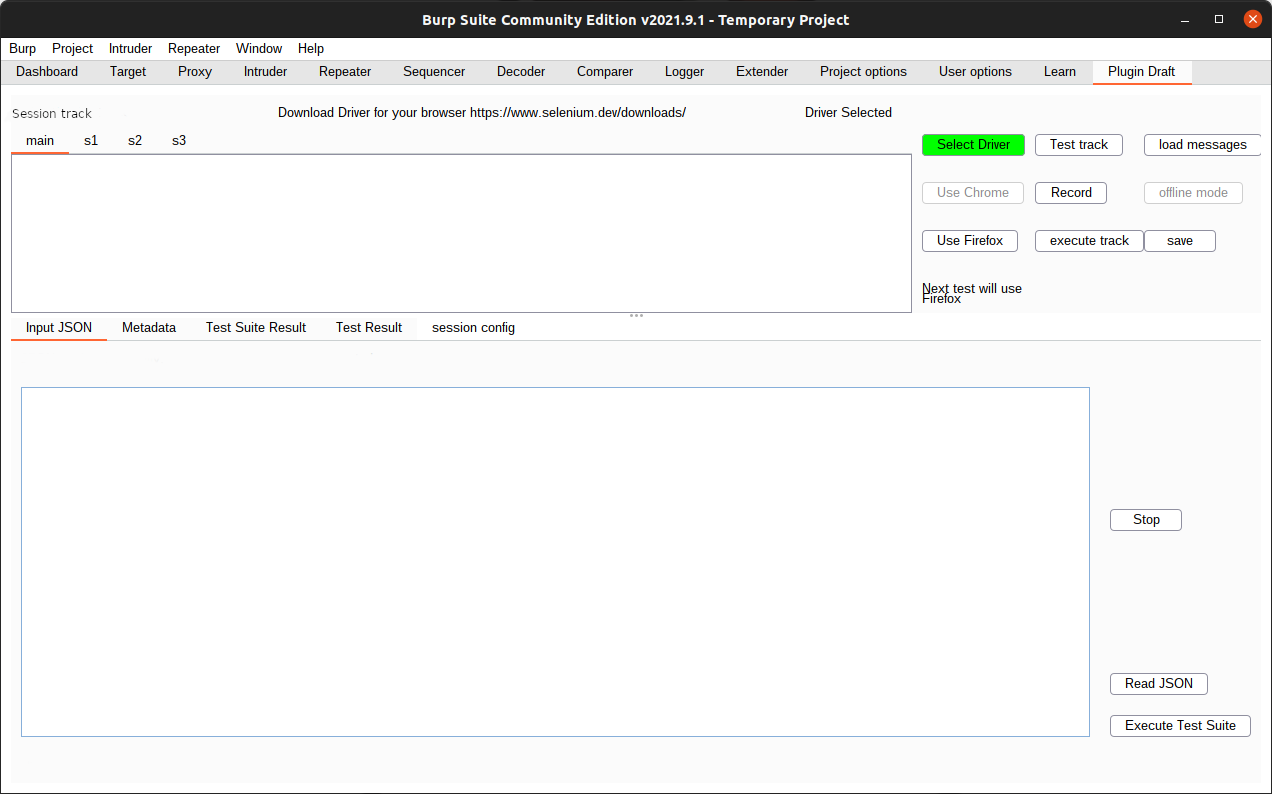
\includegraphics[width=\textwidth]{interface.png}
    \caption{Tool interface}
    \label{fig:plugin_interface}
\end{figure}

\subsection{User Interface of the tool}
In Figure \ref{fig:plugin_interface} the interface of the tool is shown, starting from top left, there is the session track input space, where it can be specified a different track for each session. Following on the top right, a series of buttons that allow various configurations can be found:
\begin{itemize}
    \item \textbf{Use Chrome} or \textbf{Use Firefox} the browser to be used can be selected
    \item \textbf{Select driver} the driver used to automate the actions on the browser can be selected
    \item \textbf{Record} the record button can be used to record the flowing messages
    \item \textbf{Load messages} the load messages button can be used to load the previously saved messages to be tested "offline"
    \item \textbf{Offline mode} the offline mode button to test the loaded messages instead of the live ones
    \item \textbf{Execute track} used to execute the session track without executing the tests, useful when the unaltered messages has to be saved.
    \item \textbf{Test track} used to test the session track without saving or doing any test.
\end{itemize}

In the bottom part multiple tabs can be found:
\begin{itemize}
    \item \textbf{Input JSON} tab is used to load the tests written in the language into the tool, and with the use of two buttons the language can be parsed, and the tests can be executed.
    \item \textbf{Test suite result} is the tab containing all the results of the executed tests
    \item \textbf{Test result} is the tab used to see the specific test result, with all the intercepted messages related to it
    \item \textbf{Session config} is used to configure the ports of the sessions that will be used in the tests.
\end{itemize}

In the bottom right part, when the \textbf{Input JSON} tab is selected, three buttons are available:
\begin{itemize}
    \item \textbf{Stop} used to stop the current execution
    \item \textbf{Read JSON} used to read the written Tests
    \item \textbf{Execute Test Suite} used to execute the written tests
\end{itemize}

\subsection{Session managing}
The sessions are managed independently, each session is basically a browser that is launched when a session is started. Each session can follow a different \gls{session track} defined in the apposite tabs. Every session is run in a separated thread to make parallelism between every session possible. By the use of specific commands in the language, is possible to do some actions on each session, like stop it, pause it, or clear its cookies. Each browser uses a different proxy port, so that it is possible to know from which session the messages come from, and so, being able to specific sessions in the tests.

\subsection{Test execution}
The test execution differs from passive to active, as passive tests do not need the edit of the messages, the execution of the \gls{session track} is done once, the messages are saved and the tests are executed on the saved messages. I have also added the possibility of exporting the saved messages to a file, in a way that they can be imported in the tool and tested again.
On the other hand, active tests needs to edit the messages, so the execution of the track has to be repeated for each test.

\subsection{Decoding \& encoding of parameters}
As said in Chapter \ref{chap:Design}, the decoding and encoding of parameters is possible. To do that, a list of encodings to be done on the parameter has to be provided, e.g., url, base64, deflate. Once the specified message is intercepted, the parameter is taken and decoded following the order of the provided encodings list. To do that, part of the code of SAML Raider \cite{saml_raider} has been used. SAML Raider is a \Gls{burp}'s plugin used to manage \Gls{SAML} certificates. The part of the code which deals with encoding and decoding of the parameters has been taken and edited to fit the tool.

\subsection{SAML certificate managing}
In \Gls{SAML} Requests and responses there is sometime the need to remove or edit the certificate associated to that request or response, so, to speed up the process a specific tag in the language has been added to remove or edit the certificate signature. There is still the possibility of doing the same removal by editing the \Gls{SAML} request or response with a regex, but with the use of the tag this becomes more convenient.
In order to do this, a part of the code of SAML Raider \cite{saml_raider} has been used, and edited to fit the needs of the tool.

\section{Problems and limitations encountered}
\label{sec:limitations}
During the implementation and the testing of the tool multiple problems have been encountered, the majority of them have been solved, but some are still present. The most relevant ones will be discussed next:

\subsection{Automation problems}
One of the biggest limitations that the tool has, is the session track actions automations, it often happens that some captcha is encountered during execution, making impossible to proceed. Moreover, the track execution is limited, there is only a possible flow of actions (the one defined) and there is not the possibility of inserting if then else constructs that could help to differentiate the actions based on the actual page or popup. For example, it could happen that a "limited time offer" popup could appear in a website only in a particular time, the execution of the session track could be compromised by that, making impossible to distinguish whether the test failed because of the tested vulnerability or the actual popup.
Another problem in the automation part of the tool is that is sometimes limited, because the session track has to been defined over a specific website, doing a set of action that is directly correlated to the website. Whenever the website is changed somehow, for example the IDs or the position of some button to be clicked change, the execution will fail, because the track could not continue.
This is still not resolved, as no methods to make the track more dynamic has been found yet. This also means that every different web service which has to be tested will need a different session track to be defined. Making it a bit time-consuming to do. 

\subsection{Oracle is sometimes ambiguous}
There still is a problem with the Oracle, where sometimes false positives or negatives arise if the execution of the tool is interrupted for any reason. This is a problem because the interruption of the execution is a term of valuation for the Oracle, this means that the oracle will give a result also based on the correctness or incorrectness of the execution of the \gls{session track}. This makes impossible to distinguish if the \gls{session track} has failed because on an error on the definition on it, or because of an expected reason (like after a message modification).

\subsection{Interface and user feedbacks}
The interface of the tool is a bit raw, it is not very user-friendly, the user experience could be improved. During my work I did not focus my attention to these topics, but they are very important as the tool is not so easy to use. Also, the feedbacks of the errors encountered by the tool such as execution errors or others are not all shown to the user, this surely has to be fixed, making more clear to the end user what is going wrong.

\subsection{Message filtering could be improved}
The message filtering part of the language could be extended by the use of an AI, making it possible to define a more abstract filter that does not solely rely on the search of parameters or exact strings.







